%
% 1_herleitung.tex -- Herleitung der Methode
%
% (c) 2025 Roman Cvijanovic & Nicola Dall'Acqua, Hochschule Rapperswil
%
% !TEX root = ../../buch.tex
% !TEX encoding = UTF-8
%

\section{Herleitung der Methode\label{neuronal:section:herleitung}}
\kopfrechts{Herleitung der Methode}

Im Folgenden wird die Methode zur Lösung von Feldgleichungen mittels eines neuronalen Netzes theoretisch hergeleitet.
Dazu wird eine allgemeine Form für Feldgleichungen bzw. partielle Differentialgleichungen benötigt.
Die allgemeine Form einer Feldgleichung lautet
\begin{equation}
\mathcal{D}(\varphi(x, t)) = 0 \qquad x \in \Omega, \quad t \in [0,T].
\label{neuronal:generelle_feldgleichung}
\end{equation}
Dabei gilt die Randbedingung
\begin{equation}
\varphi(x, t) = 0 \qquad x \in \partial \Omega, \quad t \in [0,T]
\end{equation}
sowie die Anfangsbedingungen
\begin{equation}
\varphi(x, t = 0) = f(x) \qquad x \in \Omega 
\label{neuronal:anfangsbedingung_voll}
\end{equation}
\begin{equation}
\partial_t \varphi(x, t = 0) = g(x) \qquad x \in \Omega.
\label{neuronal:anfangsbedingung_partiel}
\end{equation}


Hierbei ist:
\begin{itemize}
    \item $\varphi(x, t)$ das gesuchte Feld,
    \item $\mathcal{D}$ ein beliebiger Differentialoperator auf $\varphi$ (siehe \eqref{neuronal:bsp_differentialoperator} für ein Beispiel),
    \item $f(x)$ und $g(x)$ bekannte Funktionen, die die Anfangsbedingungen definieren,
    \item $\Omega$ das Gebiet, in dem das Feld definiert ist,
    \item $\partial \Omega$ der Rand des Gebietes,
    \item $[0,T]$ das betrachtete Zeitintervall.
\end{itemize}

Die Randbedingung legt fest, wie sich das Feld $\varphi(x, t)$ am Rand des Bereichs $\Omega$ verhält.
In diesem Fall wird angenommen, dass das Feld am Rand verschwindet, was bedeutet, dass $\varphi(x, t) = 0$ für alle $x$ auf dem Rand $\partial \Omega$ gilt.
Randbedingungen sind entscheidend, um die Lösung der Feldgleichung eindeutig zu machen, da sie die Werte des Feldes an den Grenzen des Definitionsbereichs festlegen.


Die Anfangsbedingungen beschreiben den Zustand des Feldes zu Beginn des betrachteten Zeitintervalls.
Die erste Anfangsbedingung \eqref{neuronal:anfangsbedingung_voll}, gibt die Form des Feldes zum Zeitpunkt $t = 0$ an.
Die zweite Anfangsbedingung \eqref{neuronal:anfangsbedingung_partiel}, beschreibt die zeitliche Änderung des Feldes zum Zeitpunkt $t = 0$.
Diese Bedingungen sind notwendig, um die Dynamik des Feldes über die Zeit hinweg zu bestimmen.

Der Differentialoperator $\mathcal{D}$ könnte z.B. 
\begin{equation}
    \mathcal{D}(\varphi(x, y, t)) = \frac{\partial^2 \varphi}{\partial t^2} - c^2 \left( \frac{\partial^2 \varphi}{\partial x^2} + \frac{\partial^2 \varphi}{\partial y^2} \right)
    \label{neuronal:bsp_differentialoperator}
\end{equation}
sein, setzt man dies in die Gleichung \eqref{neuronal:generelle_feldgleichung} ein, erhält man die Wellengleichung in zwei Dimensionen.

Das Ziel dieses Papers ist es, die Lösung $\varphi(x, t)$ mit einem neuronalen Netzwerk $\hat{\varphi}(x, t; \vartheta)$ zu approximieren.
Das Netzwerk verfügt über einen Vektor \( \vartheta \in \mathbb{R}^n \) von \emph{trainierbaren Parametern}.
Diese Parameter sollen so gewählt werden, dass das neuronale Netzwerk $\hat{\varphi}(x, t; \vartheta)$ die gesuchte Funktion $\varphi(x, t)$ möglichst genau approximiert.

\subsection{Aufbau neuronaler Netzwerke}\label{neuronal:subsection:struktur_nn}
In diesem Abschnitt wird erläutert, was neuronale Netzwerke sind und wie sie aufgebaut sind.
Grundsätzlich bestehen neuronale Netzwerke aus der Verkettung mehrerer Teilfunktionen:

\begin{equation}
    \hat{\varphi}(x, t; \vartheta) = f_j \circ \ldots \circ f_i \ldots \circ f_1(x, t).
    \label{neuronal:nn_ausformuliert}
\end{equation}

Jede Teilfunktion \( f_i \) setzt sich aus einer affinen Transformation und einer anschliessenden nicht-linearen Aktivierungsfunktion \( g_i \) zusammen:

\begin{align*}
    f_i\colon \mathbb{R}^q & \longrightarrow \mathbb{R}^p \colon \quad v \longmapsto g_i(A_i v + b_i)
\end{align*}

Hierbei ist \( v \in \mathbb{R}^q \), \( A_i \in \mathbb{R}^{p \times q} \) und \( b_i \in \mathbb{R}^p \). 
Die Elemente aller Matrizen \( A_i \) und Vektoren \( b_i \) bilden den Vektor \( \vartheta \) der \emph{trainierbaren Parameter} des Netzwerks.
Die Aktivierungsfunktion \( g_i \) wird elementweise auf das Ergebnis der affinen Transformation angewendet.
Die Wahl der Aktivierungsfunktion hängt stark von der zu approximierenden Funktion ab und kann beispielsweise der hyperbolische Tangens sein.

Die Definitions- und Wertebereiche der Teilfunktionen \( f_i \) sind flexibel wählbar. 
Es genügt, dass der Wertebereich jeder Teilfunktion \( f_I \) eine Teilmenge des Definitionsbereichs der nachfolgenden Teilfunktion \( f_{i+1} \) ist.
% jedoch muss der Wertebereich einer jeden Teilfunktion \( f_i \) mit dem Definitionsbereich der nachfolgenden Teilfunktion \( f_{i+1} \) übereinstimmen.
Zudem sind der Definitionsbereich der ersten Teilfunktion und der Wertebereich der letzten Teilfunktion strikt vorgegeben. 
Zur Approximation der Lösung der Feldgleichung, müssen diese Bereiche \( \mathbb{R}^2 \) bzw. \( \mathbb{R} \) sein.

Weiter ist die Anzahl der Teilfunktionen nicht strikt vorgegeben. 
Allgemein gilt, dass die Komplexität des zu approximierenden Problems die Grösse des neuronalen Netzwerks bestimmt: Je komplexer die Funktion, desto grösser muss das Netzwerk sein.

Im Abschnitt \ref{neuronal:section:rechenbeispiel} werden konkrete Definitionen für neuronale Netzwerke zur Lösung der Wellengleichung und der Burgers-Gleichung beschrieben.
Der Source-Code dieser Netzwerke ist im GitHub-Repository des Seminars verfügbar \cite{neuronal:github_source_code}.

Nachfolgend ein Beispiel für die Implementierung eines neuronalen Netzwerks mit zwei Teilfunktionen mit der Python-Bibliothek PyTorch:

\begin{lstlisting}
import torch.nn as nn
# Definition des Netzwerks
t1 = nn.Linear(2, 10)  # Affine Transformation mit Input: R^2, Output: R^10
t2 = nn.Linear(10, 1)
activation = nn.Tanh()

# Auswerten an einem gegebenen Input x
temp = activation(t1(x))
out = activation(t2(temp))
\end{lstlisting}

\subsection{Formulierung als Optimierungsproblem}\label{neuronal:subsection:optimierungsproblem}
In diesem Abschnitt wird die Wahl der \emph{trainierbaren Parameter} $\vartheta$ des neuronalen Netzwerks behandelt.
Die Auswahl von $\vartheta$ stellt im Wesentlichen ein Minimierungsproblem dar.
Die grundlegende Idee besteht darin, eine Funktion \( L(\vartheta) \) zu definieren, die den Approximationsfehler des Netzwerks quantifiziert.
Anschliessend wird diese Funktion minimiert, um die optimalen Parameter $\vartheta$ zu finden, die eine bestmögliche Approximation ermöglichen.

Um \( L(\vartheta) \) zu konstruieren, werden die Feldgleichung und die Anfangs- und Randbedingungen zunächst umgeformt.
Alle Terme werden auf eine Seite gebracht und anschliessend quadriert, um positive Fehlerwerte zu erhalten.
Für die Feldgleichung ergibt dies
\begin{equation}
    \left(\mathcal{D}(\varphi(x, t))\right)^2 = 0 \qquad x \in \Omega, \quad t \in [0,T].
    \label{neuronal:feldgleichung_umformuliert}
\end{equation}
Analog werden die Anfangsbedingungen
\begin{equation}
    \begin{aligned}
        \left(f(x) - \varphi(x, t = 0)\right)^2 = 0 \qquad x \in \Omega\\
        \left(g(x) - \partial_t \varphi(x, t = 0)\right)^2 = 0 \qquad x \in \Omega
    \end{aligned}
    \label{neuronal:anfangsbedingung_umformuliert}
\end{equation}
und die Randbedingung
\begin{equation}
    \begin{aligned}
        \left(\varphi(x, t)\right)^2 = 0 \qquad x \in \partial \Omega, \quad t \in [0,T]
    \end{aligned}
    \label{neuronal:randbedingung_umformuliert}
\end{equation}
umformuliert.
Anschliessend wird das neuronale Netzwerk $\hat{\varphi}$ für $\varphi$ substituiert
\begin{equation}
    \begin{aligned}
        &\left(\mathcal{D}(\hat{\varphi}(x, t; \vartheta))\right)^2 \qquad \qquad \quad x \in \Omega, \quad t \in [0,T]\\
        &\left(f(x) - \hat{\varphi}(x, t = 0; \vartheta)\right)^2 \qquad x \in \Omega\\
        &\left(g(x) - \partial_t \hat{\varphi}(x, t = 0; \vartheta)\right)^2 \quad \: x \in \Omega\\
        &\left(\hat{\varphi}(x, t; \vartheta)\right)^2 \qquad \qquad \qquad \: \: x \in \partial \Omega, \quad t \in [0,T].
    \end{aligned}
    \label{neuronal:umformuliert_nn}
\end{equation}
Ziel ist es, $\vartheta$ so zu wählen, dass alle diese Terme möglichst nahe bei 0 liegen.
Anders ausgedrückt, soll $\vartheta$ so gewählt werden, dass die Terme minimiert werden.

Es ist wichtig zu beachten, dass die Terme für alle $x$ und $t$ in den jeweiligen Bereichen minimal werden sollen.
Daher müssen $x$ und $t$ diskretiert werden, bevor $L(\vartheta)$ definiert werden kann.

\subsection{Diskretisierung}\label{neuronal:subsection:diskretierung}
Für die Diskretisierung werden drei Datensätze benötigt
\begin{equation}
    \begin{aligned}
        F &\subset \{\, (x, t) \,|\, x \in \Omega \setminus \partial \Omega\,, t \in (0,T] \,\}\\
        A &\subset \{\, (x, t) \,|\, x \in \Omega \setminus \partial \Omega\,, t = 0 \,\}\\
        B &\subset \{\, (x, t) \,|\, x \in \partial \Omega\,, t \in [0, T] \,\}.
    \end{aligned}
\end{equation}
Jeder Datensatz besteht aus den Punkten $k_F, k_A, k_B$, die aus einer Gleichverteilung in den jeweiligen Bereichen stammen.
Es gelten:
\begin{itemize}
    \item Die Feldgleichung für die Punkte in $F$
    \item Die Anfangsbedingungen für die Punkte in $A$
    \item Die Randbedingungen für die Punkte in $B$
\end{itemize}
Die Terme \eqref{neuronal:umformuliert_nn}, werden nun über die zugehörigen Datensätze summiert und gemittelt
\begin{equation}
  \frac{1}{\lvert F \rvert} \sum_{F}^{} \left(\mathcal{D}(\hat{\varphi}(x_i, t_i; \vartheta))\right)^2
    \label{neuronal:feldgleichung_umformuliert_netz_disk}
\end{equation}
\begin{equation}
    \begin{aligned}
        \frac{1}{\lvert A \rvert} \sum_{A}^{} \left(f(x_i) - \hat{\varphi}(x_i, t_i = 0; \vartheta)\right)^2\\
        \frac{1}{\lvert A \rvert} \sum_{A}^{} \left(g(x_i) - \partial_t \hat{\varphi}(x_i, t_i = 0; \vartheta)\right)^2
    \end{aligned}
    \label{neuronal:anfangsbedingung_umformuliert_netz_disk}
\end{equation}
\begin{equation}
    \begin{aligned}
        \frac{1}{\lvert B \rvert} \sum_{B}^{} \left(\hat{\varphi}(x_i, t_i; \vartheta)\right)^2 &.
    \end{aligned}
    \label{neuronal:randbedingung_umformuliert_netz_disk}
\end{equation}
Diese Terme hängen nur noch von $\vartheta$ ab und sollen nach wie vor möglichst gleich 0 sein.
Durch Addition der obigen Terme kann nun \( L(\vartheta) \) wie folgt definiert werden
\begin{equation}
    \begin{aligned}
        L(\vartheta) =\quad &\frac{1}{\lvert F \rvert} \sum_{F}^{} \left(\mathcal{D}(\hat{\varphi}(x_i, t_i; \vartheta))\right)^2\\
        + &\frac{1}{\lvert A \rvert} \sum_{A}^{} \left(\left(f(x_i) - \hat{\varphi}(x_i, t_i = 0; \vartheta)\right)^2
        + \left(g(x_i) - \partial_t \hat{\varphi}(x_i, t_i = 0; \vartheta)\right)^2\right)\\
        + &\frac{1}{\lvert B \rvert} \sum_{B}^{} \left(\hat{\varphi}(x_i, t_i; \vartheta)\right)^2.
    \end{aligned}
    \label{neuronal:optimierung}
\end{equation}
Für jede der drei Summen in \( L \) gilt:
\begin{itemize}
    \item Je genauer die Approximation des Netzwerks, desto näher bei 0
    \item Ist die Approximation perfekt (also \( \hat{\varphi} = \varphi \)) ist die Summe gleich 0
\end{itemize}
Dies bedeutet, je näher \( L \) bei 0 ist, desto besser ist die Approximation des Netzwerks.
$L$ ist daher tatsächlich ein Mass für den Approximationsfehler des Netzwerks.
Genauer gesagt, ist $L$ der mittlere Fehler über alle Datenpunkte der Diskretisierung.

Die Wahl der Parameter des neuronalen Netzwerks ist nun ein Minimierungsproblem:
\begin{aufgabe}
    Minimiere $L(\vartheta)$, wobei das $\vartheta$ am Minimum für die Approximation geeignet ist.
\end{aufgabe}

\subsection{Lösen des Minimierungsproblems}\label{neuronal:subsection:lösen_optimierungsproblem}
\( L \) lässt sich aus zwei Gründen nicht analytisch minimieren:
\begin{enumerate}
    \item \( L \) hängt von \( \vartheta \in \mathbb{R}^n \) ab. 
    Es müssten also alle \( n \) partiellen Ableitungen berechnet und nullgesetzt werden. 
    Da \( n \) eine sehr grosse Zahl ist, lässt sich das resultierende Gleichungssystem kaum lösen (siehe \ref{neuronal:section:rechenbeispiel} für konkrete Werte von $n$).
    \item Zudem würde das Lösen dieses Gleichungssystems voraussetzen, dass man die Feldgleichung löst, da diese in $L$ vorkommt.
\end{enumerate}
Das bedeutet, dass stattdessen ein numerischer Algorithmus verwendet werden muss.

\begin{aufgabe}
    Algorithmus (Gradientenabstieg)
    \begin{enumerate}
        \item Initialisiere \( \vartheta_1 \) mit Anfangswerten.
        \item \textbf{Schleife} von \( i = 1 \) bis \( i = m - 1 \):
        \begin{description}
            \item Berechne neue Parameterwerte: \( \vartheta_{i+1} = \vartheta_i - \varepsilon \nabla_\vartheta L\left(\vartheta_i\right) \). (Erklärung unten)
        \end{description}
        \item Gebe die Parameter \( \vartheta_m \) zurück.
    \end{enumerate}
    \label{neuronal:gradient_descent}
\end{aufgabe}

In diesem Paper wird in jedem Durchlauf des Algorithmus zusätzlich der aktuelle Wert \( L(\vartheta_i) \) berechnet.
Der Algorithmus wird beendet, sobald sich der Wert von \( L \) über mehrere Iterationen nur noch minimal ändert.

Dieser Algorithmus basiert auf dem Verhalten des Gradienten.
Der Gradient von $L$ -- ausgewertet an einem beliebigen Punkt -- ist ein Vektor, der in die Richtung des stärksten Anstiegs auf $L$ zeigt.
Durch das Minus in der Formel geht man in die entgegengesetzte Richtung, wo es wahrscheinlich abwärts geht.
Mit $\varepsilon$ wird die Schrittgrösse gesteuert, um zu verhindern, dass ein Minimum überschritten wird.

Abbildung~\ref{fig:gradientenabstieg_beispiel} veranschaulicht ein exemplarisches Beispiel eines Gradientenabstiegs.
Der Startpunkt wurde willkürlich beim grünen Punkt gewählt.
Der rote Punkt markiert ein Minimum, während die schwarz gestrichelte Kurve den Verlauf des Gradientenabstiegs darstellt.

Nach Abschluss dieses Algorithmus ist das neuronale Netzwerk mit den Parametern \( \vartheta_m \) vollständig trainiert.

\begin{figure}
    \centering
    \hspace*{-0.1\textwidth}
    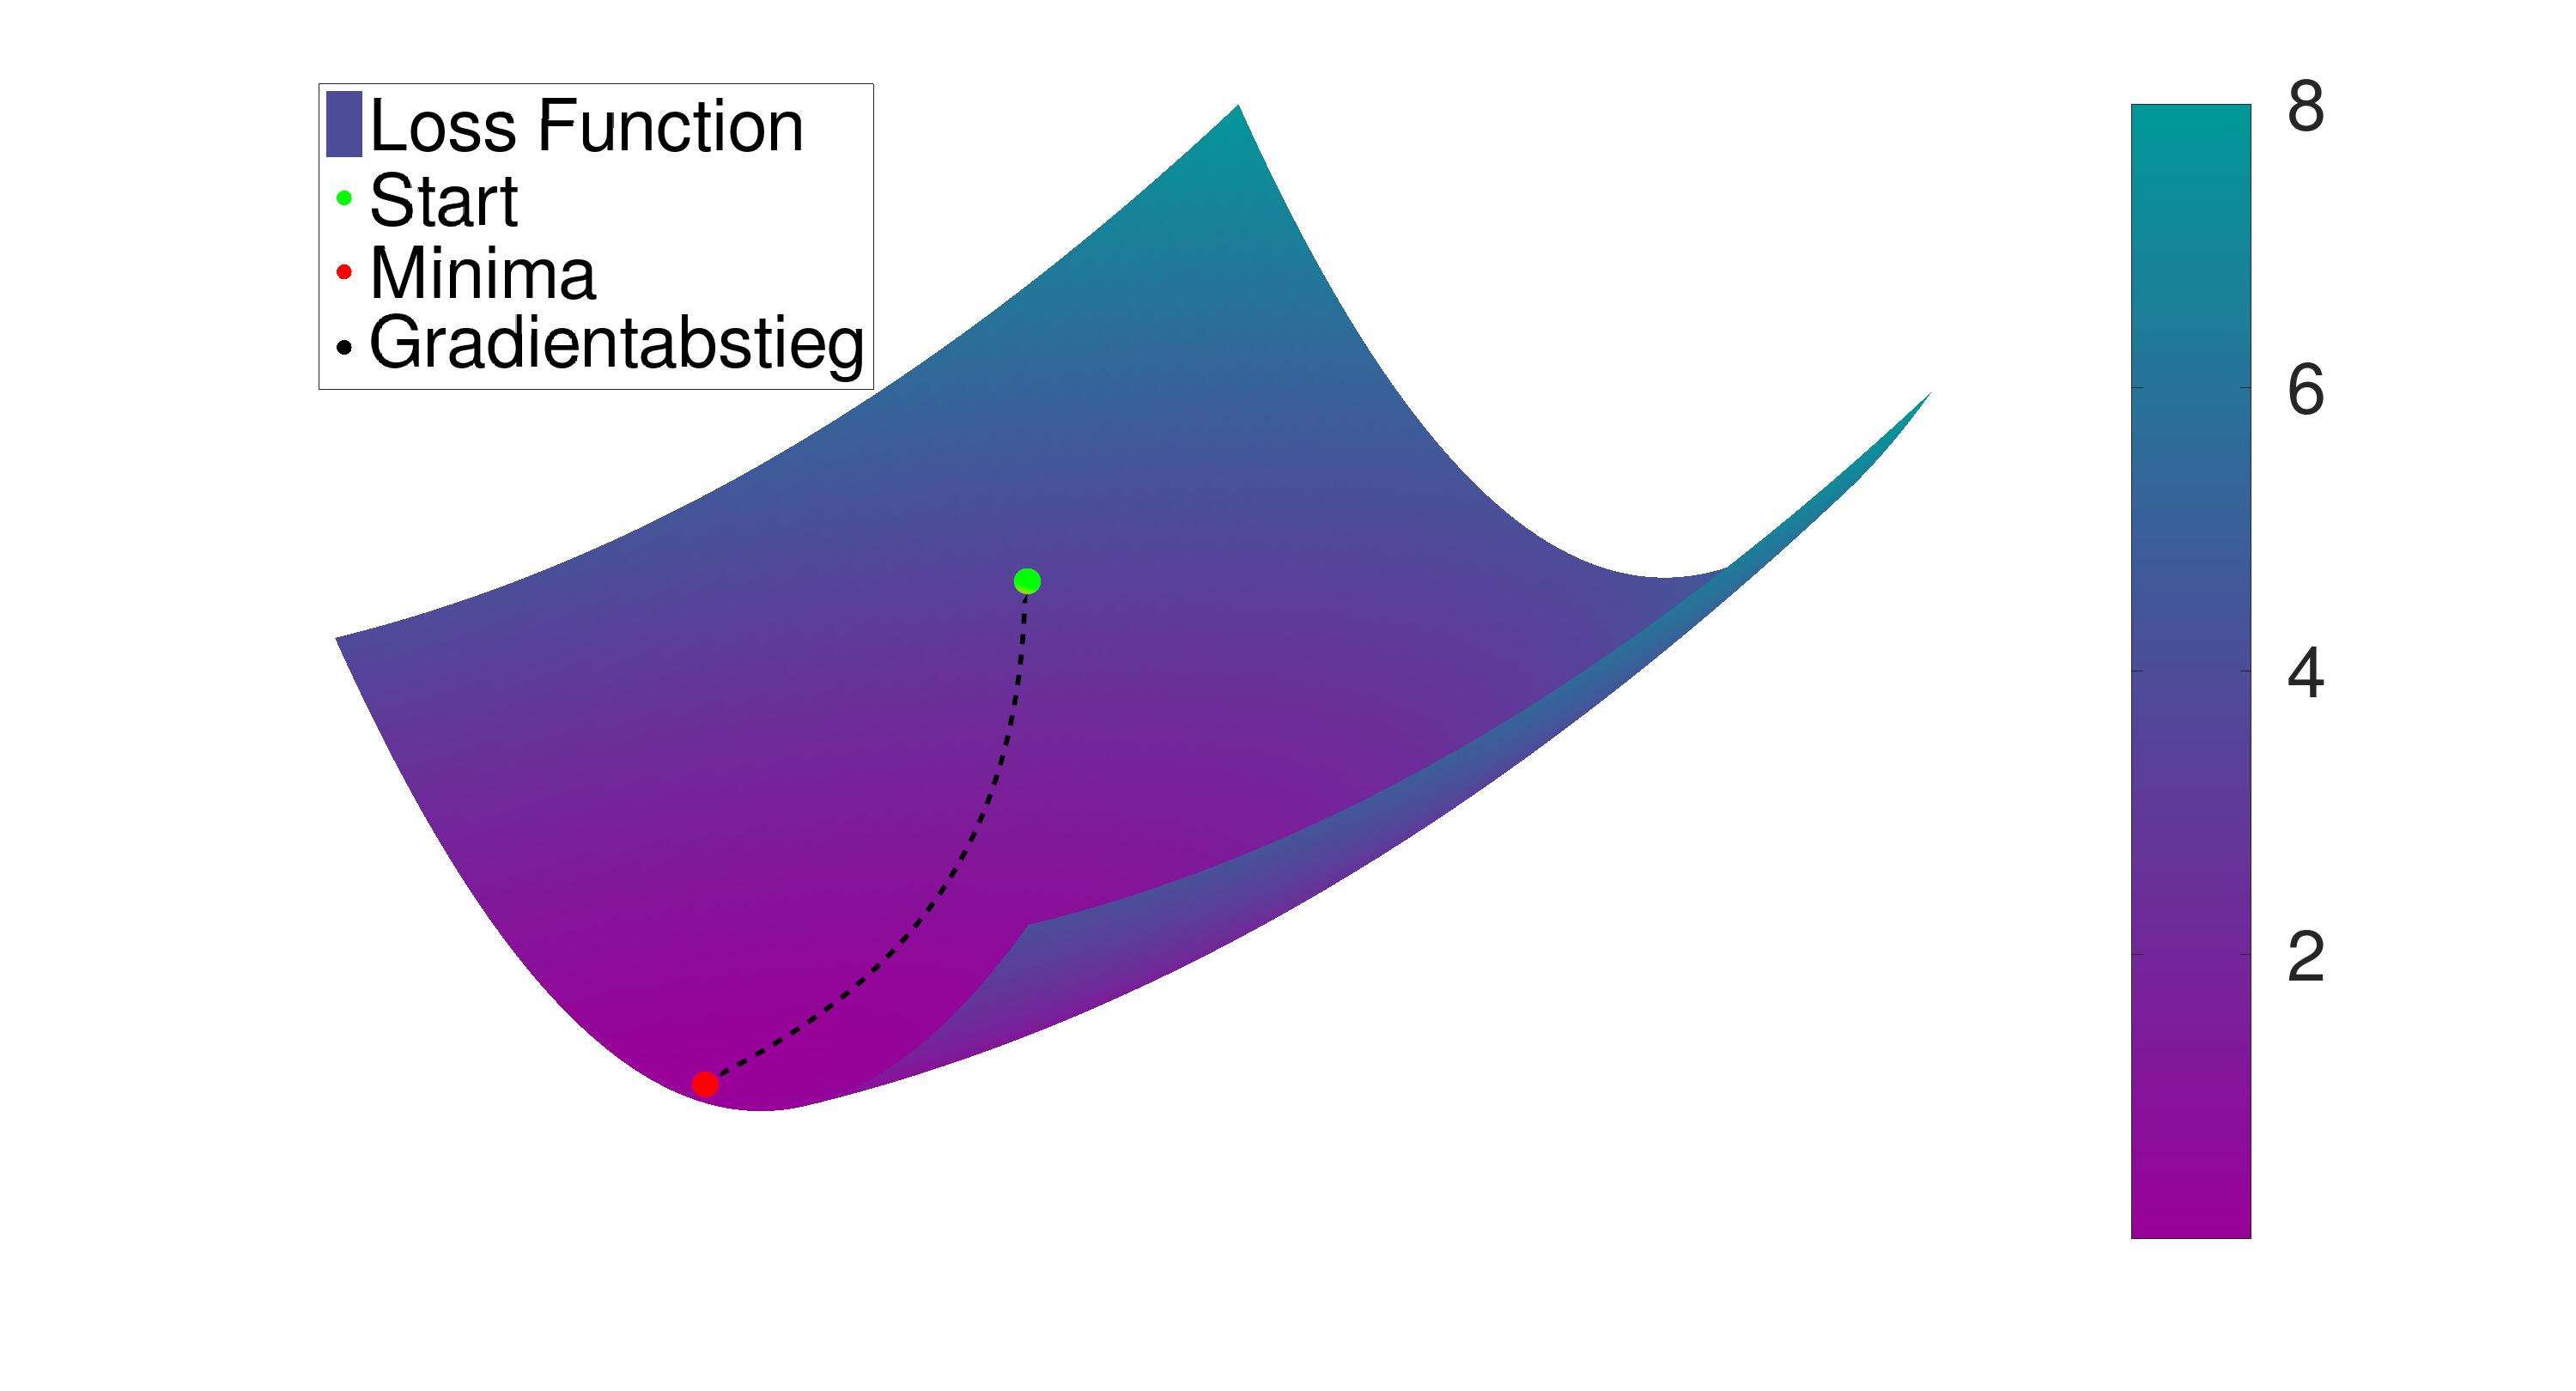
\includegraphics[width=0.9\textwidth]{papers/neuronal/images/gd_close_to_minima_long_distances_with_line.png}
    \caption{Beispiel eines Gradientenabstiegs zu einem lokalen Minimum}
    \label{fig:gradientenabstieg_beispiel}
\end{figure}


\subsubsection{Grenzen des Optimierungsverfahren}\label{neuronal:subsubsection:optimierungsverfahren_grenzen}

Der Algorithmus passt die Parameter des neuronalen Netzwerks schrittweise an, um die Funktion \( L(\vartheta) \) zu minimieren. 
Dieses Vorgehen birgt gewisse Risiken:
\begin{itemize}
    \item \textbf{Lokale Minima:} Der Algorithmus kann in einem lokalen Minimum stecken bleiben, insbesondere bei Funktionen mit vielen lokalen Minima.
    \item \textbf{Sattelpunkte und Maxima:} Der Algorithmus kann auf Sattelpunkten oder Maxima landen, wo der Gradient ebenfalls null ist und keine weitere Bewegung möglich ist.
\end{itemize}

Lokale Minima sind nicht unbedingt ein Problem. 
Ist der Wert von $L$, bzw. der Approximationsfehler, an einem lokalen Minimum sehr tief, kann dies ausreichend zur Approximation sein.

Sattelpunkte und Maxima sind ein grösseres Problem, jedoch ist es unwahrscheinlich dass der Algorithmus einen solchen Punkt findet.
Grund dafür ist, dass der Algorithmus genau auf diesen Punkten landen müsste.
Ein bisschen daneben bedeutet dass es eine Richtung gibt, in die es abwärts -- und somit weg von diesen Punkten -- geht.

\subsection{Qualitätsbewertung}\label{neuronal:subsection:qualitätsbewertung}
Für die Beurteilung der Qualität der Approximation bietet sich zunächst der Wert von \( L(\vartheta) \) nach Abschluss des Optimierungsalgorithmus an.
Dieser Wert entspricht dem mittleren Approximationsfehler, der bei den Datenpunkten aus der Diskretisierung auftritt.

Eine weitere Möglichkeit ist es, die drei Datensätze aus \ref{neuronal:subsection:diskretierung} in je zwei Teile aufzuteilen
\begin{equation*}
    \begin{aligned}
        F &= F_t \cup F_k\\
        A &= A_t \cup A_k\\
        B &= B_t \cup B_k.
    \end{aligned}
\end{equation*}
In der Funktion $L(\vartheta)$ wird über die drei Teil-Datensätze mit Index $t$ summiert.
Zudem wird eine neue Funktion \( L^1(\vartheta) \) analog zu $L(\vartheta)$ definiert, mit dem Unterschied, dass nun über die drei Teil-Datensätze mit Index $k$ summiert wird.
Da diese Funktion nie explizit durch den Optimierungsalgorithmus minimiert wurde, dient sie als Mass für den mittleren Approximationsfehler bei Datenpunkten, die nicht in der Diskretisierung enthalten waren.
Damit dies gilt muss sichergestellt werden, dass $F_t \cap F_k = \emptyset$ ist (analog für $A$ und $B$), ansonsten ist $L^1(\vartheta)$ nicht unabhängig von $L(\vartheta)$.

Eine letzte Möglichkeit zur Qualitätsbewertung ist der direkte Vergleich mit Lösungen, die durch alternative Verfahren gefunden wurden.
Existiert beispielsweise eine analytische Lösung der Feldgleichung oder wurde eine Lösung durch die Finite-Elemente-Methode gefunden, kann damit verglichen werden.
